\section{Message Passing GNN}
The message passing GNN layer captures the essence of a GNN. It is the most potent form of a GNN, but it is very expensive to implement - in terms of memory and processing. Thus, they are limited to smaller graphs. 

In message passing GNNs, each node first calculates its message and sends it to its neighbours. Each node then aggregates - the aggregation function depending on the implementation - all the messages that it received from its neighbours. The state of that node is then updated. These happen in lock step across the graph i.e. the state of each node in the graph is updated over time, in each "clock tick". An overview is shown in Figure \ref{Message_Passing_Steps} (page \pageref{Message_Passing_Steps}). 

\begin{quote}
    Note : In certain graph, the edges can be of different types. The edges themselves influence the message that is generated between two nodes
\end{quote}

\begin{figure}
     \centering
     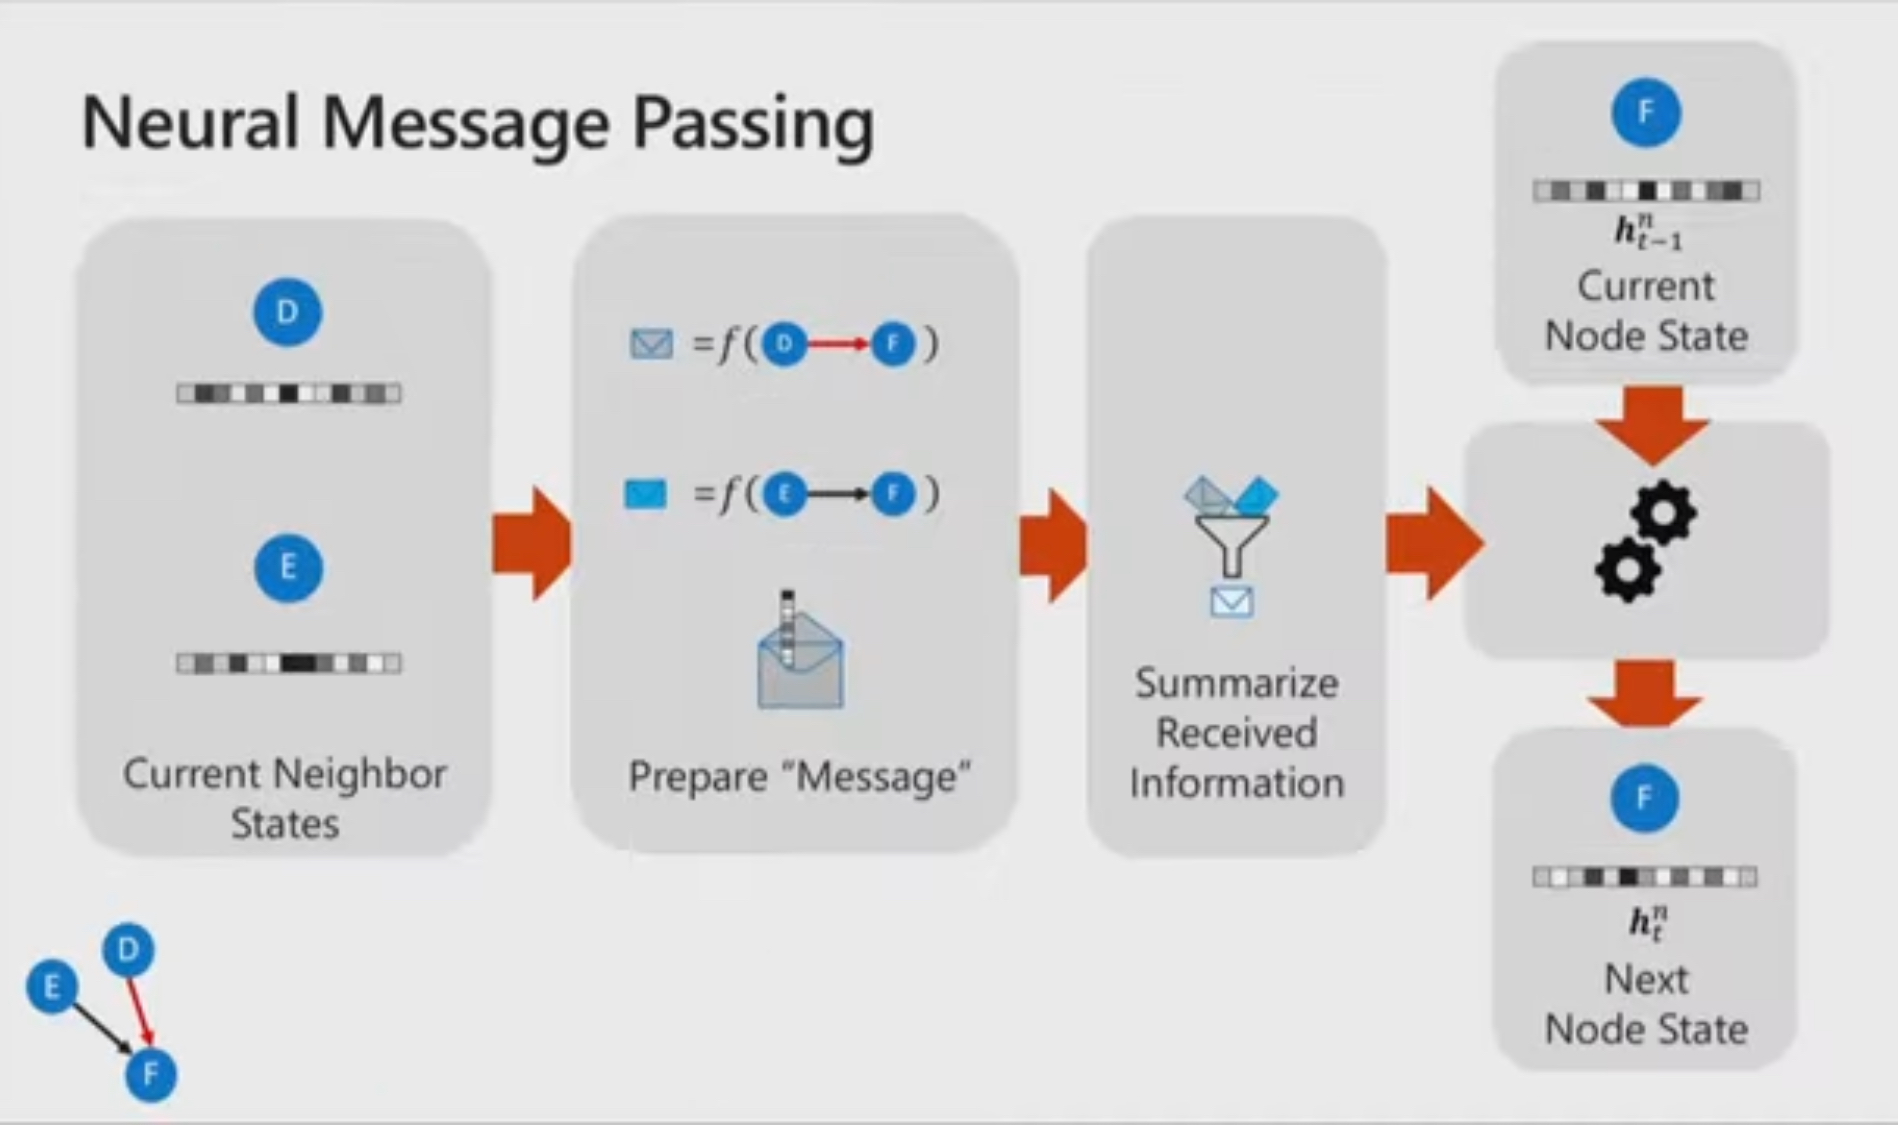
\includegraphics[width= \textwidth]{pics/Message_Passing_Steps.jpg}
     \caption{Dataflow in a Message Passing GNN Layer \cite{noauthor_introduction_nodate}}     \label{Message_Passing_Steps}
     %add_ref
\end{figure}

The change in a node's state can be described using the following equation - 
\begin{displaymath}
 h_t^{n}  = q(h_{t-1}^{n}, {\bigcup_{\forall n_{j} : n_j \xrightarrow{k} n} {f_t(h_{t-1}^{n}, k, h_{t-1}^{n_j}}))
\end{displaymath}

where, $h_t^{n}$ is the state of node $n$ at time $t$. $q$ is a non-linear transformation function. $\bigcup$ is any commutative and permutation invariant operation to combine the messages. $f_t$ is the function that produces the messages according to the previous state of node $n_j$ and node $n$ and edge type $k$. Here, $f_t$ can be dependent on time, but not necessarily.



